\documentclass[11pt]{article}
\usepackage[top=1cm, bottom=2cm, left=1cm, right=1cm]{geometry}
\usepackage{ctex}
\usepackage{algorithm}
\usepackage{algorithmicx}
\usepackage{algpseudocode}
\usepackage{amsthm,amsmath,amssymb}
\usepackage[colorlinks=true,linkcolor=blue]{hyperref}
\usepackage{listings}
\usepackage{xcolor,xparse}
\usepackage{realboxes}
\usepackage{graphics}
\usepackage{graphicx}
\usepackage{mathrsfs}
\usepackage{wrapfig}
\usepackage{subfigure}
\usepackage{pifont}
\newcommand{\To}{\textbf{To} }
\definecolor{cmdbg}{rgb}{0.9,0.9,0.9}
\lstset{%
	basicstyle=\ttfamily,
	breaklines = true,
	backgroundcolor=\color{cmdbg},
}
\DeclareDocumentCommand{\ccmd}{v}{% 参数 v 表示工作方法类似于 \verb
    \Colorbox{cmdbg}{\csname lstinline\endcsname!#1!}%
}

\makeatletter
\newenvironment{breakablealgorithm}
  {% \begin{breakablealgorithm}
   \begin{center}
     \refstepcounter{algorithm}% New algorithm
     \hrule height.8pt depth0pt \kern2pt% \@fs@pre for \@fs@ruled
     \renewcommand{\caption}[2][\relax]{% Make a new \caption
       {\raggedright\textbf{\ALG@name~\thealgorithm} ##2\par}%
       \ifx\relax##1\relax % #1 is \relax
         \addcontentsline{loa}{algorithm}{\protect\numberline{\thealgorithm}##2}%
       \else % #1 is not \relax
         \addcontentsline{loa}{algorithm}{\protect\numberline{\thealgorithm}##1}%
       \fi
       \kern2pt\hrule\kern2pt
     }
  }{% \end{breakablealgorithm}
     \kern2pt\hrule\relax% \@fs@post for \@fs@ruled
   \end{center}
  }
\makeatother

\author{谢昀城 22307110070}
\title{计算物理作业5}

\begin{document}
\maketitle


\section{题目1:五点法二阶导数公式}
\subsection{题目描述}
Derive the five-point formula for the second-order derivative.

\subsection{解答}
\[
f_{i+1} = f_i + f'_i h + \frac{1}{2} f''_i h^2 + \frac{1}{6} f'''_i h^3 + \frac{1}{4!} f^{(4)}_i h^4 + \frac{1}{5!}f^{(5)}h^5+O(h^6) \quad(1)
\]
\[
 \quad f_{i-1} = f_i - f'_i h + \frac{1}{2} f''_i h^2 - \frac{1}{6} f'''_i h^3 + \frac{1}{4!} f^{(4)}_i h^4 -\frac{1}{5!}f^{(5)}h^5+O(h^6) \quad(2)
\]

\[
f_{i+1} + f_{i-1} = 2f_i + f''_i h^2 + \frac{1}{12} f^{(4)}_i h^4 + O(h^6) \quad (3)
\]
同样的,有:
\[
f_{i+2}+f_{i-2}=2f_i+4f''_i h^2 + \frac{4}{3} f^{(4)}_i h^4 + O(h^6) \quad (4)
\]
组合(3),(4)以消去$f^{4}_i$项得到:
\[
Bf_{i+2}+Af_{i+1}+Af_{i-1}+Bf_{i-2}=2(A+B)f_i+(A+4B)f''_i h^2 +\frac{1}{6}(A+16B)+O(h^6) \quad (5)
\]
令$A+16B=0$,取$B=-1,A=16$
所以得到:
\[
f''_i={30f_i+f_{i+2}-16f_{i+1}-16f_{i-1}+f_{i-2}\over 12h^2}+O(h^4)
\]


  \section{题目3}
  \subsection{题目描述}
  The radial wave function of the 3s orbital is:
\[
R_{3s}(r) = \frac{1}{9\sqrt{3}} \times \left(6 - 6\rho + \rho^2\right) \times Z^{3/2} \times e^{-\rho/2},
\]
where:
\begin{itemize}
    \item \( r \) = radius expressed in atomic units (1 Bohr radius = 52.9 pm)
    \item \( e \approx 2.71828 \)
    \item \( Z \) = effective nuclear charge for that orbital in that atom
    \item \( \rho = \frac{2Zr}{n} \) where \( n \) is the principal quantum number (3 for the 3s orbital)
\end{itemize}

Compute
\[
\int_0^{40} |R_{3s}|^2 \, r^2 \, dr
\]
for a Si atom (\( Z=14 \)) with Simpson’s rule using two different radial grids.

\begin{enumerate}
  \item Equal spacing grids: \( r[i] = (i - 1)h; \, i = 1, \cdots, N \) (try different \( N \))
  
  \item A nonuniform integration grid, more finely spaced at small \( r \) than at large \( r \): 
  \[
  r[i] = r_0 (e^{t[i]} - 1); \quad t[i] = (i - 1)h; \, i = 1, \cdots, N
  \]
  (One typically chooses \( r_0 = 0.0005 \, \text{a.u.} \), try different \( N \)). (1 a.u. = 1 Bohr radius)
  
  \item Find out which one is more efficient, and discuss the reason.
\end{enumerate}


\subsection{程序描述}
在本程序中,我们首先计算均匀网格上的Simpson积分,对于$N=2m+1,m \epsilon \mathrm{N}$个在$[0,r_m],r_m=40$上的采样点构造系数向量和函数值向量:
\[
\vec{C} = 
\begin{bmatrix}
1 & 4 & 2 & 4 & 2 & \ldots & 2 & 4 & 1
\end{bmatrix}
\]
\[
\vec{F} = 
\begin{bmatrix}
f(r_0) & f(r_1) & f(r_2) & \ldots & f(r_{N-1})  & f(r_{N})
\end{bmatrix}
\]
则积分值$I={r_m \over 3N}\vec{C}\cdot\vec{F}$

    接着我们计算了按照$r(t) = r_0 (e^{t} - 1)$的方式划分非均匀网格。
    只需做换元$r(t)=r_0 (e^t-1),dr=(r+r_0)dt$,得到$f^*(t)=|R_{3s}(r(t))|^2r(t)^2(r(t)+r_0)$再对$f^*(t)$做均匀采样的Simpson积分即可。

    由于$R_{3s}$为径向波函数,其在$[0,\inf]$上积分为1,且随r增大迅速衰减, $|R_{3s}|^2 ~ 10^{-148}$次,故可认为其精确值为1,定义计算误差为$Error=log_{10}|I-1|$,本程序将计算不同$N$下两种积分方式的误差大小。

本程序源文件为integrate.py,在终端进入当前目录,使用命令python -u integrate.py运行本程序。运行时请保证Python第三方库Numpy,Matplotlib已安装。程序开发环境为Python3.12.3,可在Python3.8以上版本中运行。

\subsection{伪代码}
\subsubsection{Simpson Integrate 伪代码:}

\begin{breakablealgorithm}
  \begin{breakablealgorithm}
    \caption{intSimpson}
    \begin{algorithmic}
      \Function{intSimpson}{$f$, $xl$}
        \State \textbf{INPUT:} $f$ (function to integrate), $xl$ (array of sample points)
        \State \textbf{OUTPUT:} $intfx$ (integral approximation using Simpson's rule)
        
        \State $a \gets xl[0]$
        \State $b \gets xl[\text{end}]$
        
        \If{$\text{len}(xl) \% 2 = 0$}
          \State \textbf{Raise} ValueError('xl must have an odd number of elements')
        \EndIf
        
        \State $n \gets (\text{len}(xl) - 1) / 2$
        \State $c[1:2:\text{end}] \gets 4$
        \State $c[0:2:\text{end}] \gets 2$
        \State $c[0] \gets 1$
        \State $c[-1] \gets 1$
        
        \State $intfx \gets (\text{dot}(f(xl), c)) \cdot (b - a) / (6 \cdot n)$
        
        \State \Return $intfx$
      \EndFunction
    \end{algorithmic}
    \end{breakablealgorithm}
    
  \end{breakablealgorithm}
  
  
  \subsection{输入输出实例}

  对于本程序,运行后会生成图\ref{fig:int}和图\ref{fig:R2}为"integrate.png"和"R2.png"于当前目录下,并打印$N=101$时的积分值。程序运行截图如图\ref{fig:p2}所示。

  图\ref{fig:int}展示了均匀和非均匀采样的Simpson积分的误差随$N$的变化情况,为方便展示均取了10为底的对数。可以看到,在$N$较大时,其均为$N^{-4}$次的速度收敛(在$N>10^3$非均匀采样误差小于数值精度),但是非均匀采样误差小的多。

  我们画出被积函数图像如图\ref{fig:R2}(a)所示,可以看到被积函数值集中在0附近,而随着r的增大快速的趋于0。

  考虑非均匀采样时$r$在$[0,r_m]$上的分布$p(r)$:
  $$\int_0^{r}p(r)=\int_0^{t}{1\over t_m}dt
  \quad r_m=40,t_m=ln({r_m \over r_0 +1})$$
  得到$p(r)={1\over (r+r_0)t_m}$,如图\ref{fig:R2}(b),其随着$r$减小而增大,因此非均匀采样可以更多的采样$r=0$附近对积分值贡献更大的函数值,因而可以获得更好的结果。
 
  \begin{figure}[ht]
    \centering
    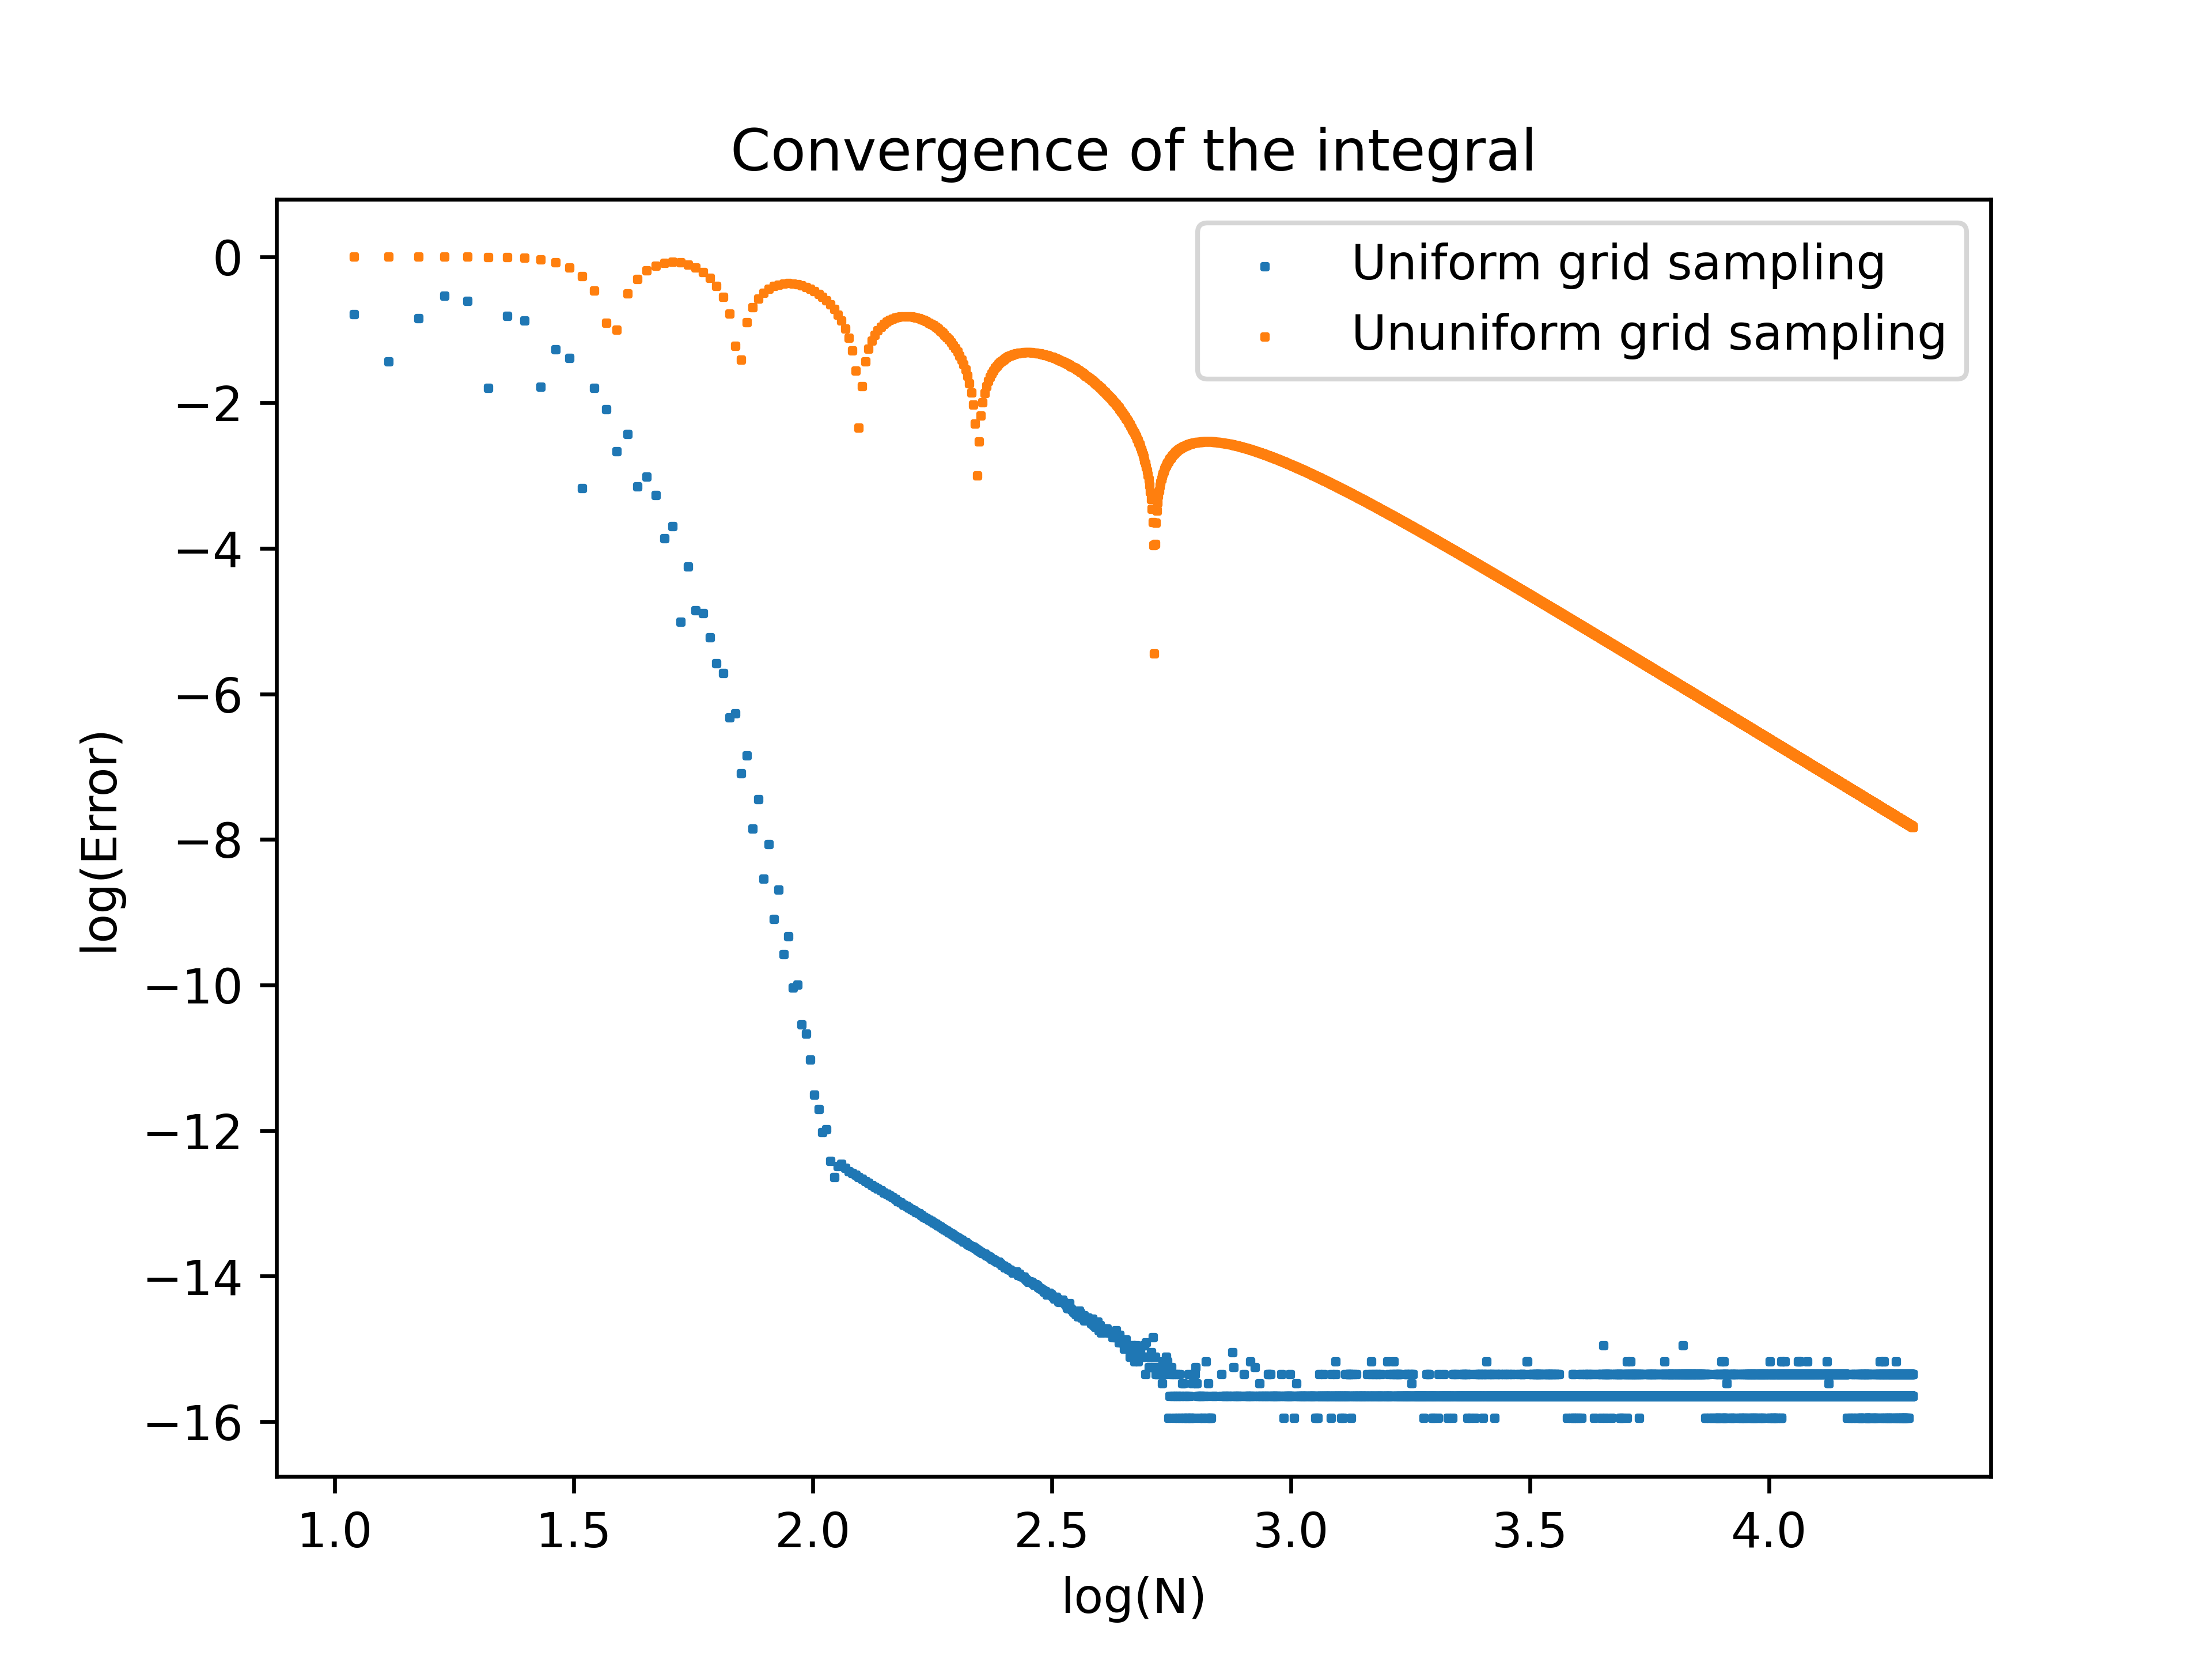
\includegraphics[width=0.8\linewidth]{photo/integrate.png}
    \caption{$V(x)=x^2$时的归一化波函数和势能}
    \label{fig:int}
  \end{figure}

  \begin{figure}[ht]
    \centering
    \includegraphics[width=1.0\linewidth]{photo/R2.png}
    \caption{(a) $|R_{3s}|^2 r^2$随$r$的变化.(b)非均匀采样时$r$的分布}
    \label{fig:R2}
  \end{figure}

  \begin{figure}
    \centering
    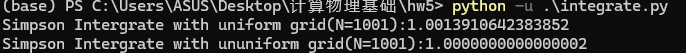
\includegraphics[width=0.6\linewidth]{photo/figp2.png}
    \caption{题目2程序运行截图}
    \label{fig:p2}
  \end{figure}


\end{document}


